\chapter{Lecture 12}
\def\over#1#2{#1}
\def\LeftRightarrow{\Leftarrow\Rightarrow}

\lhead{February 9, 2015}
\chead{21-366 Lambda Calculus Lecture 12}
\pagestyle{fancy}

\section{Untitled on Board}
\begin{equation*}
  ((\l x X)Y) \rightarrow_\beta [Y/x]X
\end{equation*}
Step 1:
\begin{equation*}
  U_1 \rightarrow_\beta \Rightarrow U_1V \rightarrow_\beta U_2V \hbox{ and } VU_1 \rightarrow_\beta VU_2
\end{equation*}
Also,
\begin{equation*}
  \l uU_1 \rightarrow_\beta \l uU_2
\end{equation*}
Many steps:
\begin{eqnarray*}
  U \rightarrow_\beta V \Rightarrow U \twoheadrightarrow_\beta V,\ U = V \Rightarrow U \rightarrow_\beta V.\\
  U_1 \twoheadrightarrow_\beta U_2 \hbox{ and } V_1 \twoheadrightarrow_\beta V_2 \Rightarrow U_1V_1 \twoheadrightarrow_\beta U_2V_2\\
\end{eqnarray*}
Additionally,
\begin{eqnarray*}
  U \twoheadrightarrow_\beta V \Rightarrow \l uU \twoheadrightarrow_\beta \l uV\\
\end{eqnarray*}

\subsection{Reduction Sequence}
\index{Reduction Sequence}
We define a reduction sequence from $U$ to $V$ as a set of $\beta$ reductions $\Delta_i$ such that
\begin{equation*}
  U = U_0 \stackrel{\Delta_0}{\rightarrow_\beta} U_1 \rightarrow_\beta \ldots \stackrel{\Delta_{n-1}}{\rightarrow_\beta} U_n = V
\end{equation*}

$U =_\beta V$ is the smallest equivalence relation\index{Equivalence Relation} $\subseteq \twoheadrightarrow_\beta$. We say that $U =_\beta V \LeftRightarrow$ there exists a sequence of terms $U_0, U_1,\ldots U_{2n}$ such that
\begin{center}
  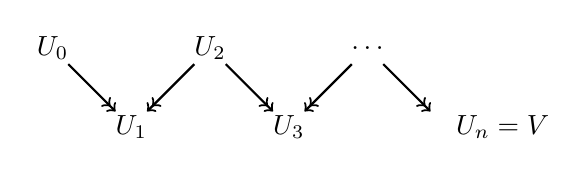
\begin{tikzpicture}
    \draw (0,0) node {$U_0$};
    \draw[->>,thick] (.2,-.2) -- (.8,-.8);
    \draw (1,-1) node {$U_1$};
    \draw[<<-,thick] (1.2,-.8) -- (1.8,-.2);
    \draw (2,0) node {$U_2$};
    \draw[->>,thick] (2.2,-.2) -- (2.8,-.8);
    \draw (3,-1) node {$U_3$};
    \draw[<<-,thick] (3.2,-.8) -- (3.8,-.2);
    \draw (4,0) node {$\ldots$};
    \draw[->>,thick] (4.2,-.2) -- (4.8,-.8);
    \draw (5,-1) node[anchor=west] {$U_{n} = V$};
  \end{tikzpicture}
\end{center}

\section{Church-Rosser Theorem}
\index{Church-Rosser Theorem|textbf}
The Church-Rosser theorem states that if there exists a term $U =_\beta V$ then there exists a $W$ such that $U \twoheadrightarrow_\beta W \twoheadleftarrow_\beta V$. We state it now without proof, but over the course of the next couple of lectures we will build up to a proof.\\

\subsection{Strong Diamond Property}
\index{Diamond Property!Strong Diamond Property|textbf}
The proof of the Church-Rosser theorem establishes something called the ``diamond property.''\index{Diamond Property} The idea is that if we can take a ``hill'' and turn it into a ``valley,'' then we can ``pave'' a sequence of beta reductions into a single valley. Formally, the diamond property states that: if
\begin{equation*}
  U \twoheadleftarrow_\beta X \twoheadrightarrow_\beta V
\end{equation*}
 
\subsection{Notes on Diagrams}
In a diagram, you see both solid lines and dotted lines. The solid lines are read ``if this line exists,'' and the dotted lines are read ``then this line exists.''
\begin{center}
  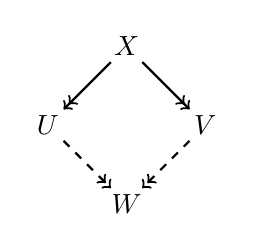
\begin{tikzpicture}
    \draw (0,0) node {$X$};
    \draw[->>,thick] (-.2,-.2) -- (-.8,-.8);
    \draw (-1,-1) node {$U$};
    \draw[dashed,->>,thick] (-.8,-1.2) -- (-.2,-1.8);
    \draw (1,-1) node {$V$};
    \draw[->>,thick] (.2,-.2) -- (.8,-.8);
    \draw (0,-2) node {$W$};
    \draw[dashed,->>,thick] (.8,-1.2) -- (.2,-1.8);
  \end{tikzpicture}
\end{center}

We can attempt to prove the strong diamond property (which is not true.) Imagine that we have $U \over{\Delta_1}{\leftarrow_\beta} X \over{\Delta_2}{\rightarrow_\beta} V$. $\Delta_1$ and $\Delta_2$ are disjoint. Notice that $\Delta_2$ has a unique residual in $U$, and $\Delta_1$ has a unique residual in $V$. We can then do:
\begin{eqnarray*}
  U \stackrel{\Delta_1}{\leftarrow_\beta} D \stackrel{\Delta_2}{\rightarrow_\beta} V\\
  U \stackrel{\Delta_2}{\rightarrow_\beta} D' \stackrel{\Delta_1}{\leftarrow_\beta} V\\
\end{eqnarray*}

Notice that
\begin{equation*}
  [Y_1/x]([Y_2/z]X_2) = [Y_1/x, [Y_1/x]Y_2/z]X
\end{equation*}

Our final case is the degenerate case $\Delta_2$ is in $Y_1$. We then have
\begin{center}
  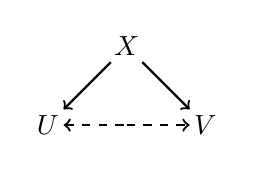
\begin{tikzpicture}
    \draw (0,0) node {$X$};
    \draw (-1,-1) node {$U$};
    \draw (1,-1) node {$V$};
    \draw[thick,->] (-.2,-.2) -- (-.8,-.8);
    \draw[thick,->] (.2,-.2) -- (.8,-.8);
    \draw[thick,dashed,->] (0,-1) -- (.8,-1);
    \draw[thick,dashed,<-] (-.8,-1) -- (0,-1);
  \end{tikzpicture}
\end{center}
So, strong diamond property does not work, but this is okay for the purposes of proving Church-Rosser. At this point in the proof, many people part ways. Church and Rosser have a proof, as do Kleene and J.J. Levy/Hindley.\\

Church and Rosser show that all of the redexes of $\Delta_2$ are disjoint. So eventually we get to our original, nondegenerate case. We will take a different route.\\

\subsection{Weak Diamond Property}
\index{Diamond Property!Weak Diamond Property|textbf}
The weak diamond property replaces the single beta reductions with beta reduction sequences:
\begin{center}
  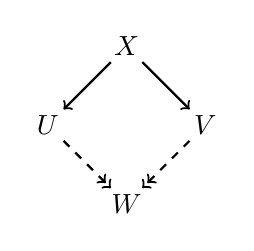
\begin{tikzpicture}
    \draw[thick,->] (-.2,-.2) -- (-.8,-.8);
    \draw[thick,dashed,->>] (-.8,-1.2) -- (-.2,-1.8);
    \draw[thick,->] (.2,-.2) -- (.8,-.8);
    \draw[thick,dashed,->>] (.8,-1.2) -- (.2,-1.8);

    \draw (0,0) node {$X$};
    \draw (-1,-1) node {$U$};
    \draw (1,-1) node {$V$};
    \draw (0,-2) node {$W$};
  \end{tikzpicture}
\end{center}
Unfortunately, the weak diamond property is not enough on its own. We cannot prove Church-Rosser using weak-diamond. Explaining why uses surjective pairings and is beyond the scope of this course.\\

\subsection{A Brief Combinatorial Fact: K\"onig's Lemma}
\index{Konig's Lemma@K\"onig's Lemma|textbf}
The German mathematician K\"onig had a theorem, called K\"onig's Lemma: a finitely branching tree with no infinite path is finite. The contrapositive is that if we have an infinite tree, then we have an infinite path.\\

\textbf{Proof:} Suppose that $T$ is an infinite, finitely branching tree. We find our infinite path in the following way. Consider all the subtrees of $T$: $T_1,\ldots T_n$. By the pidgeonhole principle, at least one of these subtrees must be infinite. Take the edge to that subtree. This finds us an infinite path. \qqed